\documentclass[tikz]{standalone}
\usepackage{pgfplots}
\pgfplotsset{compat=1.15}
\usepackage{mathrsfs}
\usetikzlibrary{arrows,calc}
\usepackage{tkz-euclide}
\pagestyle{empty}

\definecolor{AngleClr}{rgb}{0,0.39215686274509803,0}
\definecolor{ShapeClr}{rgb}{0.6,0.2,0}
\definecolor{SquareClr}{RGB}{250, 248, 217}


\begin{document}

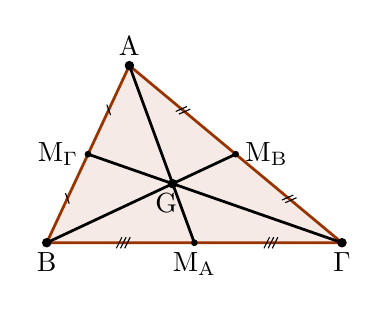
\begin{tikzpicture}[scale=.75]
\tkzSetUpLine[line width=1pt,color=black]
\tkzSetUpPoint[fill=black]

\tkzDefPoints{0/0/B,1.4/3/A,5/0/C}

\tkzDefMidPoint(B,C) \tkzGetPoint{MA}
\tkzDefMidPoint(A,C) \tkzGetPoint{MB}
\tkzDefMidPoint(A,B) \tkzGetPoint{MC}

\tkzFillPolygon[fill=ShapeClr,fill opacity=0.1](A,B,C)

\tkzInterLL(B,MB)(C,MC)
\tkzGetPoint{G}

\tkzDefPointsBy[symmetry=center G](A){}

\tkzDrawPolygon[color=ShapeClr](A,B,C)
\tkzDrawPoints[size=3](A,B,C,G)
\tkzDrawPoints[size=2](MA,MB,MC)
\tkzDrawSegments[color=black](A,MA B,MB C,MC)

\tkzLabelPoint[below](MA){$\rm M_A$}
\tkzLabelPoint[right](MB){$\rm M_B$}
\tkzLabelPoint[left](MC){$\rm M_\Gamma$}
\tkzLabelPoint[below left,xshift=0.18cm](G){$\rm G$}
\tkzLabelPoint[above](A){$\rm A$}
\tkzLabelPoint[below](B){$\rm B$}
\tkzLabelPoint[below](C){$\rm \Gamma$}

\tkzMarkSegments[mark=s|,size=2](A,MC MC,B)
\tkzMarkSegments[mark=s||,size=2](A,MB MB,C)
\tkzMarkSegments[mark=s|||,size=2](B,MA MA,C)

\end{tikzpicture}

\end{document}
